 %auto-ignore

% Aidan: maybe here put something like 'toy models of superposition proposes that the internal representations of neural networks trained on natural data are usefully represented as sparse linear combinations of features', and then 'under this assumption we can use blah blah to extract features'


Advances in artificial intelligence (AI) have resulted in the development of highly capable AI systems that make decisions for reasons we do not understand. This has caused concern that AI systems that we cannot trust are being widely deployed in the economy and in our lives, introducing a number of novel risks \citep{hendrycks2023overview}, including potential future risks that AIs might deceive humans in order to accomplish undesirable goals \citep{ngo2023alignment}. Mechanistic interpretability seeks to mitigate such risks through understanding how models calculate their outputs, allowing us to reverse engineer parts of their internal processes and make targeted changes to them \citep{christiano2021alignment, burns2022discovering, elhage2021mathematical}.
\blfootnote{Code to replicate experiments can be found at \url{https://github.com/HoagyC/sparse_coding}}

To understand a large model it is necessary to break the model down into smaller units which can be productively analysed in isolation. Using the individual neurons as these units has had some success \citep{olah2020zoom, bills2023language}, but a key challenge has been that these neurons are largely polysemantic - activating for many unrelated types of input. Also, for some model activation types (such as the residual stream of a transformer) there is little reason to expect the neurons to be a reasonable unit of analysis and massive polysemanticity is the norm.

Some recent work has attempted to solve polysemanticity by training models where it does not arise \citep{elhage2022solu}, but training fully monosemantic models is not thought to be possible \citep{anthropic2023}. Another approach focuses on specific network features that are hypothesized to exist and uses supervised probes to detect if and how the information is represented \citep{gurnee2023finding}. However, this is both difficult to scale and relies on knowing which features to expect.

\citet{elhage2022toy} investigate why polysemanticity exists and hypothesize that it is the result of models trying to represent more features than the dimension of the layer, which is made possible by the sparsity of those features in the input data. This suggests that 
Although there is uncertainty about how neural networks represent information in their internal activations, one hypothesis is that their representations are \emph{linear with superposition} \citep{elhage2021mathematical, elhage2022toy, yun2023transformer, gurnee2023finding}. This posits (1) linearity: directions in neural activation space correspond to human-understandable \textbf{network features}, and (2) superposition: that there are more network features than the layer dimension, and so network features are not all orthogonal; instead, they form an `overcomplete basis'. The linear with superposition hypothesis suggests that finding human-understandable explanations of neural networks' internal workings will involve identifying the directions that correspond to network features. We would like some method to identify these directions. 

The hypothesis that the directions form an overcomplete basis rules out the use of dimensionality reduction methods, such as Principal Component Analysis (PCA), Independent Component Analysis (ICA), or Non-negative Matrix Factorisation (NMF), since these methods are limited to finding a number of directions no higher than the dimensionality of the activation space. 

We instead build on \citet{taking_features_out_of_superposition}, who use unsupervised sparse dictionary learning \citep{olshausen1997sparse} to extract large numbers of features from the neural activations of language models. The approach is related to \citep{yun2023transformer}, who also use unsupervised dictionary learning on model activations over a text corpus to represent the model's internal activations as a sparse linear combination of neural activations (Section \ref{section:sparse_autoencoder}). Unlike Yun et al., we apply sparse coding to each layer separately, instead of to the whole residual stream and also apply it to the MLP activations. 


% Our approach, outlined in Figure \ref{fig:overview}, samples the internal activations of a language model over a text corpus, and trains an autoencoder to reconstruct these activations as a sparse linear combination of dictionary features. If we assume that network activations consist of sparse linear combinations of ground truth network features, the resulting \emph{feature dictionary} (i.e., the weight matrix of the autoencoder) should learn dictionary features that are the same direction as the ground truth network features. We can therefore attempt to interpret the dictionary features in an attempt to understand the network.


\begin{figure}
    \label{fig:overview}
    \centering
    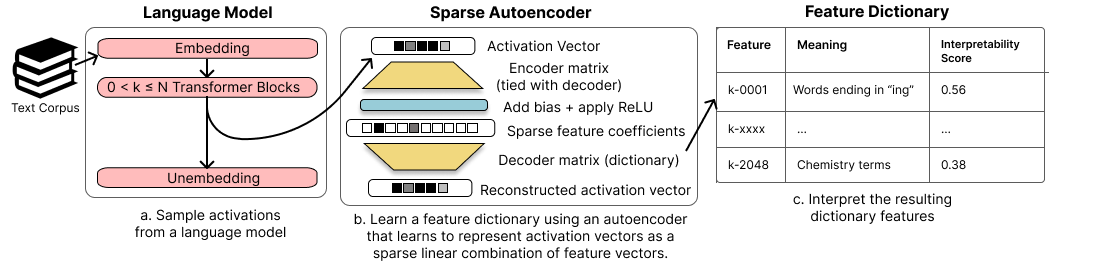
\includegraphics[width=1\textwidth]{images/sparse_coding_overview_1309.png}
    \caption{An overview of our method. We a) sample the internal activations of a language model, either the residual stream, MLP sublayer, or attention head sublayer; b) use these activations to train a neural network, a sparse autoencoder whose weights form a feature dictionary; c) interpret the resulting features with techniques such as OpenAI's autointerpretability scores.}
\end{figure}

Our features are learned without any reference to the meaning of the text, so we use several techniques to verify that our features are semantically meaningful and human-interpretable. First, we show that our features are, on average, more interpretable than other techniques as measured by autointerpretability scores \citep{bills2023language}. Next, we show that our features enable less-disruptive model concept erasure (Section \ref{section:concept_erasure}). We also show that we are able to pinpoint causally-important features for a set task (Section \ref{section:identifying_causal_features}). Finally, we provide evidence that our features are monosemantic across their activation range (Section \ref{section:monosemantic}). 